\documentclass[pdftex, a4paper,12pt]{article}

\usepackage[utf8]{inputenc}
\usepackage[T1]{fontenc}      
\usepackage{graphicx} 
\usepackage{listings}
\usepackage{color}
\usepackage{fullpage}

\lstset{ 
  basicstyle=\scriptsize,
  breaklines=true,
  showstringspaces=false
}
\parindent=0pt

\title{A Simple Linux Shell - ASH (Awesome SHell)}
\author{Andre Christensen (110033) og Jacob Pedersen (120374)}

\begin{document}

\maketitle
\newpage

\tableofcontents
\newpage

\section{Introduction}

This journal describes our implementation of a simple Linux shell, given as a mandatory lab exercise in the course `Operating Systems and Embedded Linux - IOSLX4-E13`.\\

ASH contains the following features:

\begin{itemize}
	\item Execute commands in the foreground.
	\item Execute commands (upto 20) in the background (by appending a `\&` to the command).
	\item A built-in `killbg` command which kills all processes running in the background.
\end{itemize}



\section{Implementation details}

ASH is capable of executing commands in both the foreground and in the background. Every command in read from the \emph{stdin} and parsed into tokens seperated by spaces. A `run-in-background` flag is set, if the character `\&` is appended at the end of the command.\\

After the command has been read a new child is forked, and depending on the type of process (foreground or background) the shell waits for the PID to exit, or becomes ready to accept a new command from the user.\\

ASH keeps track of background processes, by keeping their PID's in an array. The status of all background processes is checked each time the SIGCHLD signal handler is fired. Checking the status of a process implies calling \emph{waitpid} on the background process' PID with the WNOHAND flag, and checking if the system call returns the process' PID, which means the process and exited.


\section{Testing}

Figure \ref{fig:1} shows a screenshot of a testrun. The screenshots shows the following:

\begin{itemize}
	\item `ps` is executed in the foreground and lists running processes.
	\item The `./test` program is started in the background (PID 7958), and the prompt is immediately ready for input again.
	\item `ps` is executed again, and `./test` is now listed as running.
	\item The built-in `killbg` is now executed, and outputs shows that the `./test` process (PID 7958) is killed.
	\item `ps` is executed again, and shows the test program isn't running anymore.
	\item Finally the built-in `exit` command is executed, and ASH exits.
\end{itemize}

\begin{figure}[!ht]
	\centering
	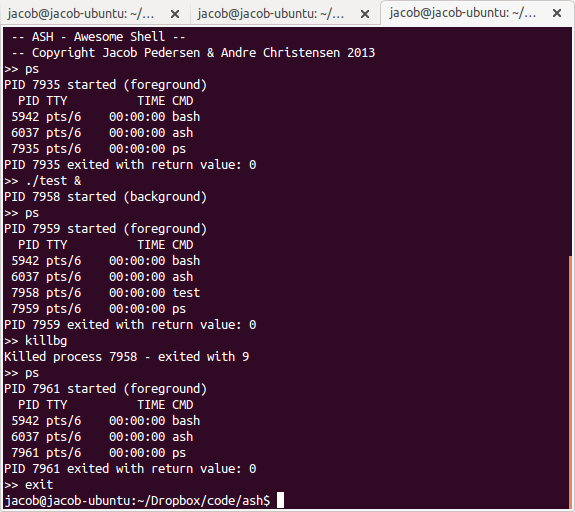
\includegraphics[width=1\textwidth]{testing}
	\caption{Execution of jobs in the foreground and background, and demonstration of the killbg command}
	\label{fig:1}
\end{figure}

\subsection{Test system details}

\begin{itemize}
	\item OS: Ubuntu 13.10 (Linux 3.11.0)
	\item Compiler: gcc 4.8.1 (Ubuntu/Linaro)
	\item Makefile: See Listing \ref{lst2}
\end{itemize}


\clearpage
\section{Source Code}

\lstinputlisting[caption=ash.c, language=C, label=lst1]{../ash.c}
\hrule
\lstinputlisting[caption=Makefile, language=make, label=lst2]{../Makefile}

\end{document}
